\chapauthor{Чертков В.М.\\Захаров В.В.\\Крищенович В.А.}
\chapter{Обеспечение информационной безопасности в рамках Экосистемы OSTIS}
\chapauthortoc{Чертков В.М.\\Захаров В.В.\\Крищенович В.А.}
\label{chapter_security}

\abstract{Аннотация к главе.}

\section*{Введение в \textit{Главу \ref{chapter_security}}}
Большое разнообразие моделей обеспечения информационной безопасности, всё возрастающий объем данных, которые необходимо анализировать для обнаружения атак на информационные системы, изменчивость методов атак и динамическое изменение защищаемых информационных систем, необходимость оперативного реагирования на атаки, нечеткость критериев обнаружения атак и выбора методов и средств реагирования на них, нехватка высококвалифицированных специалистов по защите влечет за собой потребность в использовании методов искусственного интеллекта для решения задач безопасности.

\section{Специфика обеспечения информационной безопасности интеллектуальных систем нового поколения}
Информационную безопасность интеллектуальных систем следует рассматривать с двух точек зрения:
\begin{textitemize}
	\item с точки зрения применения искусственного интеллекта в информационной безопасности;
	\item с точки зрения организация информационной безопасности в интеллектуальных системах.
\end{textitemize}

\textbf{Применения искусственного интеллекта в информационной безопасности}

Следует отметить, что искусственный интеллект активно применяется для мониторинга и анализа уязвимостей безопасности в сетях передачи информации {[}2 Исобоев{]}. Система искусственного интеллекта позволяет машинам более эффективно выполнять поставленные задачи, такие как:

\begin{textitemize}
	\item визуальное восприятие, распознавание речи, принятие решений и перевод с одного языка на другой.
	
	\item обнаружение вторжений -- искусственный интеллект может обнаруживать сетевые атаки, заражения вредоносным программным обеспечением и другие киберугрозы;
	
	\item кибераналитика -- искусственный интеллект также используется для анализа больших данных с целью выявления закономерностей и аномалий в системе кибербезопасности организации с целью обнаружения не только известных, но и ещё неизвестных угроз;
	
	\item безопасная разработка программного обеспечения -- искусственный интеллект может помочь создать более безопасное программное обеспечение, предоставляя разработчикам обратную связь в режиме реального времени.
\end{textitemize}

При этом искусственный интеллект используется не только для защиты, но и для нападения, например для эмуляции акустических, видео и других образов с целью обмана механизмов аутентификации и дальнейшей имперсонации, обман проверки человек или робот capcha и т.д.

В настоящее время можно определить следующие классы систем, в которых применяется искусственный интеллект:

\begin{textitemize}
	\item UEBA (User and Entity Behavior Analytics) -- система анализа поведения субъектов (пользователей, программ, агентов и т.д.) на предмет обнаружения нестандартного поведения и использования их для обнаружения потенциальных угроз с использованием шаблонов угроз (паттернов);
	\item TIP (Threat Intelligence Platform) -- платформы раннего обнаружения угроз на основе сбора и анализа информации индикаторов компрометации и реагирования на них. Применение методов машинного обучения повышает эффективность обнаружения неизвестных угроз на ранних этапах;
	\item EDR (Endpoint Detection and Response) -- системы обнаружения атак оперативного реагирования на конечных точках компьютерной сети. Могут обнаруживать вредоносные программы, автоматически классифицировать угрозы и самостоятельно реагировать на них;
	\item SIEM (Security Information and EventManagement) -- системы сбора и анализа информации о событиях безопасности от сетевых устройств и приложений в реальном времени и оповещения;
	\item NDR (Network Detection and Response) -- системы обнаружения атак на сетевом уровне и оперативного реагирования на них. ИИ использует накопленную статистику и базу знаний об угрозах;
	\item SOAR (Security Orchestration and Automated Response) -- системы, позволяющие выявлять угрозы информационной безопасности и автоматизировать реагирование на инциденты. В решениях данного типа, в отличие от SIEM-систем, ИИ помогает не только проводить анализ, но и автоматически реагировать надлежащим образом на выявленные угрозы;
	\item Средства защиты приложений (Application Security) -- системы, позволяющие определять угрозы безопасности прикладных приложений, управлять процессом мониторинга и устранения таких угроз;
	\item Антифрод (Antifraud) -- платформы в режиме реального времени обнаруживают угрозы в бизнес-процессах и мошеннические операции. ИИ используется для определения отклонений от идентифицированных бизнес-процессов с целью выявления вторжений или уязвимости процессов и повышает адаптивность к изменению логики и метрик бизнес-процессов.
\end{textitemize}


В работе [3 Частикова] предложена методика построения нейроиммунной системы анализа инцидентов информационной безопасности, объединяющей модули сбора и хранения (сжатия) данных, модуль анализа и корреляции событий информационной безопасности и подсистемы обнаружения сетевых атак на основе сверточных нейронных сетях. Использование технологий машинного обучения в информационной безопасности создает узкие места и системные уязвимости, которые можно использовать и имеет следующие недостатки [4 Абдурахман]:

\begin{textitemize}
	\item наборы данных, которые должны быть сформированы из значительного количества входных выборок, что требует много времени и ресурсов;
	\item требуется огромное количество ресурсов, включая память, данные и вычислительную мощность;
	\item частые ложные срабатывания, которые нарушают работу и в целом снижают эффективность таких систем;
	\item организованные атаки на основе искусственного интеллекта (семантические вирусы).
\end{textitemize}

\textbf{Организация информационной безопасности в интеллектуальных системах}

Определим цели обеспечения информационной безопасности систем нового поколения.

Из монографии А.В. Остроух [5] \textbf{целями обеспечения информационной безопасности традиционных интеллектуальных систем} являются:

\begin{textitemize}
	\item обеспечение конфиденциальности информации в соответствии с проведенной классификацией;
	\item обеспечение целостности информации на всех этапах, связанных с нею процессов (создание, обработка, хранение, передача и уничтожение) при предоставлении публичных услуг;
	\item обеспечение своевременной доступности информации при предоставлении публичных услуг;
	\item обеспечение наблюдаемости, направленной на фиксирование любой деятельности пользователей и процессов;
	\item обеспечение аутентичности и невозможности отказа от транзакций и действий, производимых участниками предоставления публичных услуг;
	\item учет всех процессов и событий, связанных с вводом, обработкой, хранением, предоставлением и уничтожением данных.
\end{textitemize}

Следует отметить так как интеллектуальные системы нового поколения будут взаимодействовать с подобными себе системами понимая при этом, о чем осуществляется запрос, то цели обеспечения будут выглядеть по-другому. \textbf{Целями обеспечения информационной безопасности интеллектуальных систем нового поколения} являются:

\begin{textitemize}
	\item обеспечение сохранности семантической совместимости информации;
	\item защита достоверности и целостности информации;
	\item обеспечение доступности информации на разных уровнях интеллектуальной системы;
	\item минимизация ущерба от событий, несущих угрозу информационной безопасности.
\end{textitemize}

В настоящее время разработаны классические подходы и принципы обеспечения безопасности баз знаний (данных), интерфейсов связи (обмена информацией) между компонентами интеллектуальных систем такие, как шифрование передаваемых данных, фильтрация ненужного (избыточного) контента и политика разграничения доступа к данным.

Система обеспечения информационной безопасности должна создаваться на следующих принципах:

\begin{textitemize}
	\item принцип равнопрочности -- означает обеспечение защиты оборудования, программного обеспечения и системы управления от всех видов угроз;
	\item принцип непрерывности -- предусматривает непрерывное обеспечение безопасности информационных ресурсов, ИС для непрерывного предоставления публичных услуг;
	\item принцип разумной достаточности -- означает применение таких мер и средств защиты, которые являются разумными, рациональными и затраты на которые, не превышают стоимости последствий нарушения информационной безопасности;
	\item принцип комплексности -- для обеспечения безопасности во всем многообразии структурных элементов, угроз и каналов несанкционированного доступа должны применяться все виды и формы защиты в полном объеме;
	\item принцип комплексной проверки -- заключается в проведении специальных исследований и проверок, специального инженерного анализа оборудования, верификационных исследований программных средств. Должен осуществляться непрерывный мониторинг аварийных сообщений и параметров ошибок, постоянно должно выполняться тестирование аппаратного и программного оборудования, а также контроль целостности программных средств, как при загрузке программных средств, так и в процессе функционирования;
	\item принцип надежности -- методы, средства и формы защиты должны надежно перекрывать все пути проникновения и возможные каналы утечки информации, для этого допускается дублирование средств и мер безопасности;
	\item принцип универсальности -- меры безопасности должны перекрывать пути угроз независимо от места их возможного воздействия;
	\item принцип плановости -- планирование должно осуществляться путем разработки детальных планов действий по обеспечению информационной защищенности всех компонент системы предоставления публичных услуг;
	\item принцип централизованного управления -- в рамках определенной структуры должна обеспечиваться организованно-функциональная самостоятельность процесса обеспечения безопасности при предоставлении публичных услуг;
	\item принцип целенаправленности -- необходимо защищать то, что должно защищаться в интересах конкретной цели;
	\item принцип активности -- защитные меры обеспечения безопасности в работе процесса предоставления услуг должны претворяться в жизнь с достаточной степенью настойчивости;
	\item принцип квалификации обслуживающего персонала -- обслуживание оборудования должно осуществляться сотрудниками, подготовленными не только в вопросах эксплуатации техники, но и в технических вопросах обеспечения безопасности информации;
	\item принцип ответственности -- ответственность за обеспечение информационной безопасности должна быть ясно установлена, передана соответствующему персоналу и утверждена всеми участниками в рамках процесса обеспечения информационной безопасности.
\end{textitemize}

\section{Принципы, лежащие в основе обеспечения информационной безопасности ostis-систем}

Архитектура Экосистемы OSTIS представлена на рисунке \textit{\nameref{fig:ecosystem_security}}.

\begin{figure}[H]
	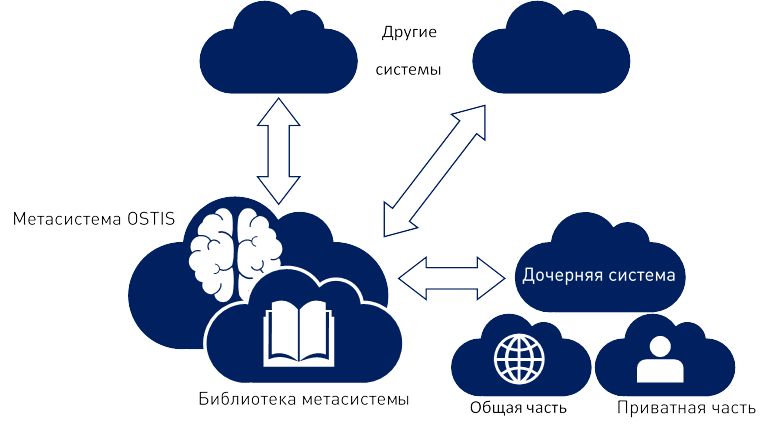
\includegraphics[scale=0.9]{images/part7/chapter_security/ecosystem_security.png}
	\caption{Архитектура Экосистемы OSTIS в контексте решения задач информационной безопасности}
	\label{fig:ecosystem_security}
\end{figure}

Экосистема OSTIS представляет собой коллектив взаимодействующих:

\begin{textitemize}
	\item ostis-систем;
	\item пользователей ostis-систем (конечных пользователей и разработчиков);
	\item других компьютерных систем, не являющихся ostis-системами, но являющихся дополнительными информационными ресурсами или сервисами для них
\end{textitemize}

Ядро \textit{Технологии OSTIS} включает следующие компоненты:
\begin{textitemize}
	\item семантическая база знаний OSTIS, которая может описывать любой вид знаний, при этом ее легко дополнять новыми видами знаний.
	\item решатель задач OSTIS основанный на подходе, в котором применяется множество агентов. Такой подход позволяет легко интегрировать и комбинировать любые модели решения задач.
	\item интерфейс OSTIS-системы, представляющий собой подсистему со своей базой знаний и решателем задач.
\end{textitemize}

Представленная архитектура Экосистемы OSTIS реализует следующие основные идеи:
\begin{textitemize}
	\item все базы знаний объединяются в Глобальную базу знаний, качество которой (логичность, корректность, целостность) постоянно проверяется множеством агентов. Все проблемы описываются в единой базе знаний, и для их устранения при необходимости привлекаются специалисты;
	\item каждое приложение, связанное с экосистемой OSTIS, имеет доступ к последней версии всех основных компонентов OSTIS, обновление компонентов выполняется автоматически;
	\item каждый владелец приложения Экосистемы OSTIS может поделиться частью своих знаний платно или бесплатно.
\end{textitemize}

В рассмотренной Экосистеме OSTIS требуется организация обеспечения информационной безопасности на каждом из уровней: обмен данными, права доступа к данным, аутентификация клиентов Экосистемы, шифрование данных, получение данных из открытых источников, обеспечение достоверности и целостности хранимых и передаваемых данных, контроль за нарушением связей в базе знаний.

Следует отметить, что для некоторых направления по обеспечению информационной безопасности семантических систем могут применяться методы и алгоритмы, разработанные в рамках традиционных интеллектуальных систем. Для интеллектуальных систем нового поколения можно выделить ряд аспектов, в рамках которых требуется работка новых алгоритмов и методов обеспечения информационной безопасности. Рассмотрим основные направления обеспечения информационной безопасности семантических интеллектуальных систем.

\textbf{Ограничение информационного трафика, анализируемого интеллектуальной системой}

Экспоненциальный рост объема информации, циркулирующей в информационных потоках и ресурсах в условиях вполне определенных количественных ограничений на возможности средств ее восприятия, хранения, передачи и преобразования формирует новый класс угроз информационной безопасности, характеризуемых избыточностью совокупного входящего информационного трафика интеллектуальных систем.

В результате переполнение информационных ресурсов интеллектуальной системы избыточной информацией может спровоцировать распространения искаженной (деструктивной семантической) информации. Общая методология защиты интеллектуальных систем от бесполезной информации осуществляется посредством использования аксиологических фильтров, реализующих функции численной оценки ценности поступающей информации, отбора наиболее ценной и отсеивания (фильтрации) менее ценной (бесполезной или вредной) с использованием вполне определенных критериев.

Следует также выделить в отдельную категорию угроз информационной безопасности активные средства разрушения семантики баз знаний (семантические вирусы) {[}6{]}.

\textbf{Политика разграничении доступа к базе знаний}

Мандатная политика безопасности (MAC -- mandatory access control) основывается на мандатном (принудительном) разграничении доступа, определяющемся четырьмя условиями: все субъекты и объекты системы идентифицируются; задается решетка уровней безопасности информации; каждому объекту системы присваивается уровень безопасности, определяющий важность содержащейся в нем информации; каждому субъекту системы присваивается уровень доступа, определяющий уровень доверия к нему в интеллектуальной системе. Кроме того, мандатная политика имеет более высокую степень надёжности. Реализация данной политики основывается на разработанном алгоритме определения согласованных уровней безопасности всех элементов онтологии.

Так как семантические базы знаний в отличие от реляционной базы данных позволяют выполнять правила для получения логических выводов, то для обеспечения безопасности данных актуальным является разработка алгоритмов и методов, с помощью которых можно будет получать только данные, имеющие уровни безопасности меньше уровней доступа субъектов их запросивших {[}7{]}.

\textbf{Связность}

Вся информация, хранимая в семантической памяти интеллектуальной системы, систематизирована в виде единой базе знаний. К такой информации относятся непосредственно обрабатываемые знания, интерпретируемые программы, формулировки решаемых задач, планы и протоколы решения задач, информация о пользователях, описание синтаксиса и семантики внешних языков, описание пользовательского интерфейса и многое другое {[}8{]}. В информационной базе знаний между фрагментами информации (единицами информации) должна быть предусмотрена возможность установления связей различного типа. Прежде всего, эти связи могут характеризовать отношения между информационными единицами. Нарушение связей приводит к неправильному логическому выводу, либо к получению ложных знаний, либо к несовместимости знаниям в базе.

\textbf{Введение семантической метрики}

На множестве информационных единиц в некоторых случаях полезно задавать отношение, характеризующее ситуационную близость информационных единиц, т.е. силу ассоциативной связи между информационными единицами {[}11{]}. Его можно было бы назвать отношением релевантности для информационных единиц. Такое отношение дает возможность выделять в информационной базе знаний некоторые типовые ситуации. Отношение релевантности при работе с информационными единицами позволяет находить знания, близкие к уже найденным.

\textbf{Семантическая совместимость}

Внутренняя семантическая совместимость между компонентами интеллектуальной компьютерной системы (т.е. максимально возможное введение общих, совпадающих понятий для различных фрагментов хранимой базы знаний), являющаяся формой конвергенции и глубокой интеграции внутри интеллектуальной компьютерной системы для различного вида знаний и различных моделей решения задач, что обеспечивает эффективную реализацию мультимодальности интеллектуальной компьютерной системы. Внешняя семантическая совместимость между различными интеллектуальными компьютерными системами, выражающаяся не только в общности используемых понятий, но и в общности базовых знаний и являющаяся необходимым условием обеспечения высокого уровня социализации интеллектуальных компьютерных систем {[}9{]}.

\textbf{Активность}

В интеллектуальной системе для актуализации тех или иных действий способствуют знания, имеющиеся в этой системе. Таким образом, выполнение активностей в интеллектуальной системе должно инициироваться текущим состоянием информационной базы знаний. Появление в базе фактов или описаний событий, установление связей может стать источником активности системы {[}10{]}. В том числе преднамеренное искажение информации и связей может стать источником преднамеренного искажения информации.

Важно отметить, что интеллектуальная информационная система нового поколения -- это самостоятельный субъект, который может сам осознанно, целенаправленно и постоянно заботиться о себе, в том числе о своей собственной безопасности.


%\input{author/references}